% #############################################################################
% This is Chapter 5
% !TEX root = ../main.tex
% #############################################################################
\providecommand{\pv}[1]{\textcolor{blue}{#1}} % provisional number: update from the final run
\fancychapter{Data-Flow Analysis}
% The following line allows to ref this chapter
\label{sec:toolkit}

The metadata of Chapter~\ref{chap:implement} describes the \emph{structure} of an application: which agents, tools, and stores it contains. The attacks of Chapter~\ref{chap:back}, however, depend on data: untrusted content that reaches a model, a tool, or a store and is then treated as instructions. This chapter describes the static data-flow analysis that measures where the inputs of an application's AI components come from. 

We first define sinks and sources (Section~\ref{sec:df-model}), then describe the architecture of the analysis (Section~\ref{sec:df-architecture}), the patterns it recognizes and why (Section~\ref{sec:df-recognition}), how it traces data (Section~\ref{sec:df-analysis}), and how traces become measurements (Section~\ref{sec:df-patterns}). We close with the validation method (Section~\ref{sec:df-validation}) and the limitations of the analysis (Section~\ref{sec:df-limitations}).

% =============================================================================
\section{Sources and Sinks}
\label{sec:df-model}

We use the source--sink formulation of static taint analysis~\cite{livshits2005,arzt2014flowdroid}. A sink is a place in the code where data enters an AI component; a source is where that data originates. The analysis is static, therefore it reads the code and never executes it.

\paragraph{Sinks.} Data enters an agentic application's AI components in three ways, through models, tools, and stores. Which gives the sink categories and types of Table~\ref{tab:df-sinks}.
Whilst the query made to a store is considered a sink, the retrieved content is considered a source, because it is data coming out of the store.

\begin{table}[t]
\centering
\footnotesize
\renewcommand{\arraystretch}{1.2}
\setlength{\tabcolsep}{4pt}
\caption{Sink categories and types.}
\label{tab:df-sinks}
\begin{tabular}{@{}>{\raggedright\arraybackslash}p{0.11\textwidth}>{\raggedright\arraybackslash}p{0.12\textwidth}>{\raggedright\arraybackslash}p{0.38\textwidth}>{\raggedright\arraybackslash}p{0.33\textwidth}@{}}
\toprule
\textbf{Category} & \textbf{Type} & \textbf{Data entering the component} & \textbf{Example} \\
\midrule
model & call & inputs of a call to a model or agent & \texttt{llm.invoke(prompt)}, \texttt{agent.run(q)} \\
      & instructions & system prompt or instructions of an agent & \texttt{Agent(instructions=...)} \\
      & history & a message added to a conversation later sent to a model & \texttt{messages.append(...)} \\
\addlinespace[2pt]
tool  & params & parameters of a function the model can call & \texttt{@tool def search(q)} \\
      & effect & a command, file, network, or database operation inside a tool whose argument the model controls & \texttt{subprocess.run(cmd)} \\
      & result & the value a tool returns to the model & \texttt{return page.text} \\
      & dispatch & code in which model output selects the function to run & \texttt{TOOLS[name](**args)} \\
\addlinespace[2pt]
store & write & content written into a vector store or agent memory & \texttt{store.add\_texts(docs)} \\
      & query & the query and filters sent to a store & \texttt{store.search(q)} \\
\bottomrule
\end{tabular}
\end{table}

\paragraph{Sources.} Each input of a sink is traced back to sources, grouped into eight classes by who controls the data (Table~\ref{tab:df-sources}). 
\emph{Primary} sources, the first 5 classes listed (Table~\ref{tab:df-sources}), introduce data into the program. \emph{Derived} sources, the remaining 3 classes, are outputs of other sinks so their own origin is found by continuing at the sink that produced them.
For the risk analysis, \texttt{user}, \texttt{external}, and \texttt{database} are \emph{untrusted} (an outside party can control them), and \texttt{external}, \texttt{store\_read}, and \texttt{tool\_result} are \emph{indirect} (content the model reads without the end user typing it), the channel of indirect prompt injection (V1).

\begin{table}[t]
\centering
\footnotesize
\renewcommand{\arraystretch}{1.2}
\setlength{\tabcolsep}{4pt}
\caption{Source classes.}
\label{tab:df-sources}
\begin{tabular}{@{}>{\raggedright\arraybackslash}p{0.14\textwidth}>{\raggedright\arraybackslash}p{0.20\textwidth}>{\raggedright\arraybackslash}p{0.58\textwidth}@{}}
\toprule
\textbf{Source} & \textbf{Controlled by} & \textbf{Examples} \\
\midrule
\texttt{constant} & developer & literals; prompt files in the repository read with a fixed path \\
\texttt{config} & deployer & environment variables, configuration files \\
\texttt{user} & end user & request bodies and parameters of HTTP handlers, chat inputs, command-line arguments \\
\texttt{external} & third party & web requests; web-search, scraping, e-mail, chat, and issue-tracker clients; files read from a non-fixed path; command output \\
\texttt{database} & whoever wrote the data & ORM and SQL reads \\
\midrule
\texttt{model} & the model & output of a model call; parameters of a tool \\
\texttt{tool\_result} & depends on the tool & value returned by a tool called from application code \\
\texttt{store\_read} & whoever wrote to the store & content retrieved from a vector store or memory \\
\bottomrule
\end{tabular}
\end{table}

\paragraph{Input classes.} From its sources, each input receives an \emph{input class}: \emph{static} if all sources are constants, \emph{deployment-fixed} if it depends only on constants and configuration, \emph{dynamic} if at least one source is determined at run time, and \emph{undetermined} if the trace could not be completed without finding a run-time source. The analysis never guesses a source it cannot see; undetermined inputs are reported as such.

% =============================================================================
\section{Architecture}
\label{sec:df-architecture}

Table~\ref{tab:df-architecture} lists the components of the analysis, in the order in which a repository passes through them, together with the main design decision behind each.

\begin{table}[t]
\centering
\footnotesize
\renewcommand{\arraystretch}{1.2}
\setlength{\tabcolsep}{4pt}
\caption{Components of the data-flow analysis and the reasons for their design.}
\label{tab:df-architecture}
\begin{tabular}{@{}>{\raggedright\arraybackslash}p{0.17\textwidth}>{\raggedright\arraybackslash}p{0.36\textwidth}>{\raggedright\arraybackslash}p{0.41\textwidth}@{}}
\toprule
\textbf{Component} & \textbf{Role} & \textbf{Design decision and reason} \\
\midrule
Acquisition & downloads each repository as a snapshot through the GitHub API and runs one analysis process per repository & The analysed commit is recorded, so every result can be reproduced; memory and time limits per process keep a single very large repository from stopping the corpus run. \\
Parsing & parses Python with Python's \texttt{ast}~\cite{python-ast} and JavaScript/TypeScript with the TypeScript compiler~\cite{typescript} & Official parsers are exact; the TypeScript syntax tree is converted into Python's representation, so both languages share one analysis. \\
Repository index & indexes files, imports (including monorepo packages and re-exports), functions, classes, and declared types & Calls are resolved the way the language resolves them---through imports, \texttt{self}, and class hierarchies---rather than by matching names across the repository, which would connect unrelated code. \\
Pattern mapping & holds every library and framework name the analysis recognizes & Framework knowledge is kept apart from the analysis logic, so frameworks can be added without changing how data is traced. \\
Object recognition & identifies models, agents, stores, external clients, and tools & A call counts as a sink only when its receiver is such an object, so generic method names (\texttt{run}, \texttt{add}, \texttt{search}) do not produce false sinks. \\
Sink detection & finds the sinks of Table~\ref{tab:df-sinks} and their inputs & Every input is traced, including arguments that are not analysed further, so the output shows what was deliberately left out. \\
Tracing & follows each input backwards to its sources & Bounded by five function boundaries and 20{,}000 visited syntax nodes per trace, which keeps the analysis tractable on large repositories. \\
Output & writes one record per repository with every sink, input, source, and trace step & Each step carries its file, line, and code, so every aggregate number can be traced back to the code that produced it. \\
Aggregation & computes tables, figures, reports, and validation samples & Kept separate from the analysis, so results can be recomputed without rescanning the corpus. \\
\bottomrule
\end{tabular}
\end{table}

% =============================================================================
\section{Recognition Patterns}
\label{sec:df-recognition}

Table~\ref{tab:df-recognition} summarizes the families of patterns the analysis recognizes, with representative examples and the reason for each. As in established static taint analyses, sources and sinks are specified as curated lists of APIs~\cite{arzt2014flowdroid,rasthofer2014susi}. The patterns were compiled from the official documentation of the frameworks in Table~\ref{tab:frameworks}, from the API tables of the pattern-based analysis (Chapter~\ref{chap:implement}), and from the misses found during validation, the complete list is given in Appendix~\ref{app:patterns}.

The recognition patterns were refined iteratively against code the analysis had not been developed on. In each round, the analysis was run on a set of ten repositories from the corpus, and its findings were compared with a manual inspection of their code: model calls, tools, and stores the inspection found but the analysis did not was examined to determine why it was missed.

Misses caused by unknown names, such as agents created through factory functions instead of constructors, web-search clients, or vector-store clients, were resolved by adding the corresponding patterns, taken from the official documentation of the framework concerned; misses caused by how a value was passed, such as models received through dependency injection or declared through type aliases, were resolved by extending how the analysis recognizes objects. 

From the API tables of the pattern-based analysis (Chapter~\ref{chap:implement}) we adopted the names of agent, model, store, and tool interfaces, as well as the external readers and tool effects of the vulnerability patterns. 

Misses that cannot be resolved by patterns, such as agents kept in framework or user-interface state, are reported as limitations (Section~\ref{sec:df-limitations}).

\textbf{Two principles apply throughout.} First, generic names count only in context: a method such as \texttt{add} or \texttt{search} is a store operation only on a recognized store object, and a method such as \texttt{all} or \texttt{first} is a database read only on a query, session, or result object (for example, JavaScript's \texttt{Promise.all} is not mistaken for one). Second, objects are recognized by three methods: from their constructors, from factories and from declared types, because many applications receive their models through dependency injection or build agents with factory functions.

\noindent
\begin{minipage}{\linewidth}
\begin{lstlisting}[language=Python, caption={Method 1 - Constructor}, label={lst:df-example}]
llm = ChatOpenAI(model="gpt-4o")
llm.invoke(prompt)               # recognised: llm comes from a known constructor
\end{lstlisting}
\end{minipage}

\noindent
\begin{minipage}{\linewidth}
\begin{lstlisting}[language=Python, caption={Method 2 - Factory Function}, label={lst:df-example}]
agent = create_react_agent(llm, tools)
agent.invoke({"messages": msgs})  # recognised: create_react_agent is a known agent factory
\end{lstlisting}
\end{minipage}


\noindent
\begin{minipage}{\linewidth}
\begin{lstlisting}[language=Python, caption={Method 3 - Declared Type}, label={lst:df-example}]
class ChatService:
    def __init__(self, llm: BaseChatModel):   # created by the framework, injected here
        self.llm = llm

    def answer(self, q):
        return self.llm.invoke(q)             # recognised: the declared type is a model type
\end{lstlisting}
\end{minipage}

\begin{table}[t]
\centering
\footnotesize
\renewcommand{\arraystretch}{1.2}
\setlength{\tabcolsep}{4pt}
\caption{Pattern families recognized by the analysis, with representative examples.}
\label{tab:df-recognition}
\begin{tabular}{@{}>{\raggedright\arraybackslash}p{0.15\textwidth}>{\raggedright\arraybackslash}p{0.44\textwidth}>{\raggedright\arraybackslash}p{0.35\textwidth}@{}}
\toprule
\textbf{Family} & \textbf{Recognized} & \textbf{Why} \\
\midrule
Model objects & constructors of LLM clients and agents (\texttt{ChatOpenAI}, \texttt{Anthropic}, CrewAI and OpenAI Agents \texttt{Agent}, \texttt{CodeAgent}, \texttt{ConversableAgent}); agent and chain factories (\texttt{create\_react\_agent}, \texttt{createToolCallingAgent}); declared types (\texttt{BaseChatModel}); derived objects (\texttt{bind\_tools}, \texttt{as\_query\_engine}) & Calls on these objects are model sinks. Many applications create agents through factory functions or receive models through injection, not through a constructor. \\
Model calls & SDK methods (\texttt{chat.completions.create}, \texttt{messages.create}); SDK functions (\texttt{generateText}, \texttt{streamText}); invocation methods on model objects (\texttt{invoke}, \texttt{run}, \texttt{kickoff}, \texttt{initiate\_chat}); agent-to-agent messages (\texttt{A2AClient.send\_message}) & Covers both direct SDK use and framework agents. \\
Instructions & keyword arguments such as \texttt{system\_prompt}, \texttt{instructions}, \texttt{system\_message} & Text that the model treats with developer authority. \\
Tools & decorators (\texttt{@tool}, \texttt{@function\_tool}, \texttt{@mcp.tool}); factories and registrations (\texttt{StructuredTool.from\_function}, \texttt{tool(\{execute\})}, \texttt{server.registerTool}); \texttt{tools=[...]} lists & Tool parameters are chosen by the model. \\
Tool effects & \emph{exec}: \texttt{subprocess}, \texttt{eval}, \texttt{child\_process}; \emph{fs}: \texttt{open}, \texttt{fs.writeFile}, \texttt{shutil}; \emph{net}: \texttt{requests}, \texttt{fetch}, \texttt{axios}; \emph{db}: \texttt{execute} & The consequence classes of unauthorized actions and data leakage (R5, R6)~\cite{owasp}, corresponding to command and code injection~\cite{cwe-78,cwe-94}, path traversal~\cite{cwe-22}, server-side request forgery~\cite{cwe-918}, and SQL injection~\cite{cwe-89}; code execution reached from model output is a known source of vulnerabilities in LLM-integrated applications~\cite{liu2024llmsmith}. \\
Stores & vector-store and memory classes (Chroma, Qdrant, Pinecone, Weaviate, Mem0, Zep, LangGraph stores), their factories (\texttt{from\_documents}), collections and indexes derived from them, and sub-interfaces (\texttt{zep.memory}); write and read methods on these objects & Generic method names are meaningful only on store objects; stores are the target of memory and RAG poisoning~\cite{poisonedrag,agentpoison}. \\
Sources & \emph{config}: \texttt{os.getenv}, \texttt{process.env}; \emph{user}: request fields, parameters of HTTP handlers, chat inputs; \emph{external}: HTTP clients and web-search, scraping, e-mail, chat, and issue-tracker clients (and objects they return); \emph{database}: ORM and SQL reads & Determine who controls each input; third-party content is the channel of indirect prompt injection~\cite{greshake}. \\
Heuristic & invocation methods on any object created by a known LLM framework package & Catches agents of frameworks without a precise rule; reported separately. \\
\bottomrule
\end{tabular}
\end{table}

% =============================================================================
\section{Tracing}
\label{sec:df-analysis}

For every input of every sink, the analysis traces the value backwards through assignments, string formatting and concatenation, containers (lists, dictionaries, message objects), function parameters to the arguments at their call sites, return values of called functions, constants imported from other files, and attributes of objects and classes. When a trace stops without reaching a source, the reason is recorded (for example, a parameter of a function that is never called within the repository).

A trace crosses at most five function boundaries: enough to follow the typical path in an application from an entry point through a service and helper functions to the call that sends a prompt, while preventing traces from fanning out through large call graphs, where the number of paths grows exponentially with depth. Together with a budget of 20{,}000 visited syntax nodes per trace, this keeps the analysis tractable on large repositories. Branches cut off by either limit are reported as undetermined, never as constant, so the limits can only make the results more conservative.

Retrieved content is handled differently, because it comes out of a store rather than out of code. Writes and reads are linked when they refer to the same store object, and the retrieved content inherits the sources of the content written into that store. When no write is found in the repository, typically because the store is filled by a separate ingestion service, its origin is undetermined.
\paragraph{Detection levels.} Sinks are detected at two levels of confidence. 
\begin{itemize}
    \item \emph{Confirmed} sinks are found by the precise patterns of Table~\ref{tab:df-recognition}: a known SDK function (\texttt{client.chat.completions.create}, \texttt{generateText}), or a method called on an object that the analysis has recognized as a model or agent through its constructor (\texttt{ChatOpenAI(...)}), a factory (\texttt{create\_react\_agent(...)}), or a declared type (\texttt{llm: BaseChatModel}).
    \item \emph{Heuristic} sinks extend detection to frameworks and classes without a precise rule: a call of a typical invocation method (\texttt{invoke}, \texttt{run}, \texttt{stream}, \texttt{chat}) on any object created from a known LLM framework package. Because the analysis does not know which arguments of such a call carry content, it traces all of them, and instruction-like keyword arguments such as \texttt{prompt} are counted as instructions. The heuristic thus finds agents that the precise rules miss, such as those of frameworks released after the patterns were compiled but may also include calls that are not model calls.
\end{itemize}
Confirmed results are therefore the main results, and results including heuristic sinks are reported separately as an upper bound; keeping the two apart raises recall without mixing in the lower precision of the heuristic.

\paragraph{Example.} In Listing~\ref{lst:df-example}, the parameter \texttt{file} of an MCP tool is model-controlled; it reaches \texttt{fs.readFileSync}, a file-system \emph{effect}; and the file's content is returned to the model, a tool \emph{result} with source \texttt{external}. A model manipulated through its input can thus read any file accessible to the server, and the content flows back into the model.

\paragraph{Example.} Listing~\ref{lst:df-example} shows the three tool sinks in one MCP tool. The parameter \texttt{file} is chosen by the model (tool \emph{parameter}, source \texttt{model}); it reaches \texttt{fs.readFileSync}, a file-system operation (tool \emph{effect}); and the file's content is returned to the model (tool \emph{result}, source \texttt{external}). A model manipulated through its input can thus read any file accessible to the server, and the content flows back into the model.

\noindent\begin{minipage}{\linewidth}
\begin{lstlisting}[language=JavaScript, caption={The three tool sinks in an MCP tool (illustrative).}, label={lst:df-example}]
server.registerTool("read", { description: "read a file" },
  async ({ file }) => {                           // tool parameter: chosen by the model
    const text = fs.readFileSync(file, "utf8");   // tool effect (fs): model controls the path
    return { content: [{ type: "text", text }] }; // tool result: file content returns to the model
  });
\end{lstlisting}
\end{minipage}

% =============================================================================
\section{Measurements and Risk Patterns}
\label{sec:df-patterns}

All results are reported at the level of repositories: a repository counts once for a property, however often the property occurs in its code. Counting values instead would let a few very large repositories dominate the results. Each share is reported relative to the repositories in which the property can occur at all; for example, only repositories that call a model can pass untrusted content to a model.

\paragraph{Sinks and inputs (RQ2).} For each sink type we report its prevalence and the input classes of its inputs, and for each source class which sink types it reaches. For source classes we also report \emph{reach}: the share of a source's occurrences that flow into at least one sink. Most occurrences of environment reads, file reads, and request fields occur in parts of an application that have nothing to do with AI, so reach is computed over files that contain an AI sink, plus sources elsewhere that reach a sink.


\paragraph{Risk patterns (RQ3).} Five patterns capture the preconditions of the attack vectors of Chapter~\ref{chap:back} (Table~\ref{tab:df-patterns}). A repository matches a pattern if it occurs at least once in its code. The patterns describe \emph{exposure}---the data flow an attack requires is present---not exploitability, since sanitization, authentication, and model behavior are not analysed.

Figures~\ref{fig:risk-direct}--\ref{fig:risk-store} illustrate how the patterns are detected. The first three patterns require a single data flow: a source of the listed classes reaching the sink (Figure~\ref{fig:risk-direct}). The tool risk combination requires two conditions in the same repository, which may be met by different tools (Figure~\ref{fig:risk-tool}). The store poisoning chain is followed across three steps: from an untrusted write into a store, through a read of that same store, to a model call (Figure~\ref{fig:risk-store}).

\begin{figure}[t]
  \centering
  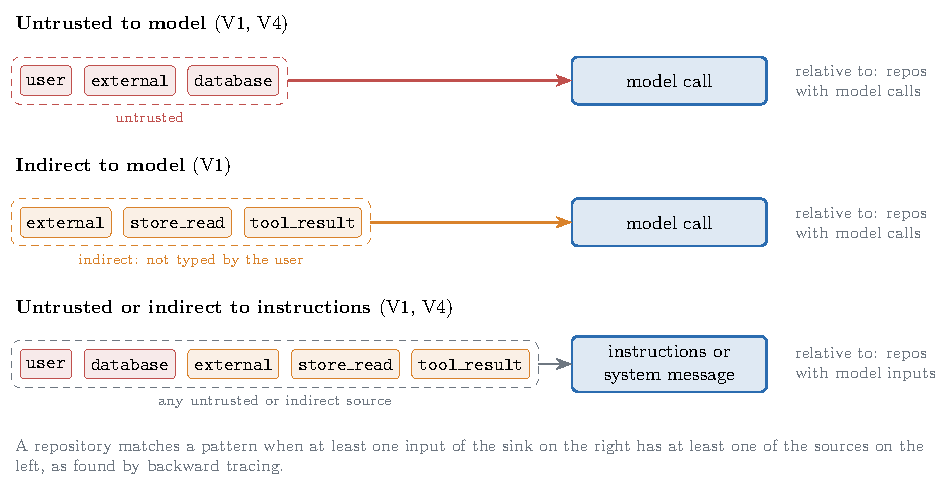
\includegraphics[width=\linewidth]{Images/flow/risk_patterns_direct.pdf}
  \caption{Detection of the three direct risk patterns: a repository matches when at least one input of the sink has one of the listed sources.}
  \label{fig:risk-direct}
\end{figure}

\begin{figure}[t]
  \centering
  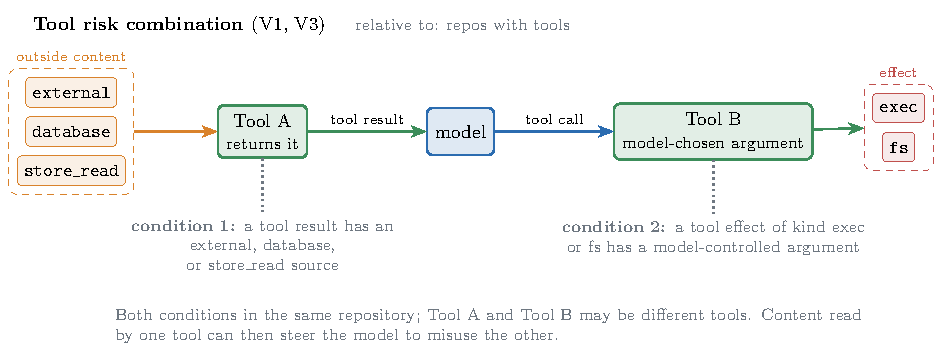
\includegraphics[width=\linewidth]{Images/flow/risk_tool_combination.pdf}
  \caption{Detection of the tool risk combination: a tool returns outside content to the model, and a tool lets the model execute commands or access files.}
  \label{fig:risk-tool}
\end{figure}

\begin{figure}[t]
  \centering
  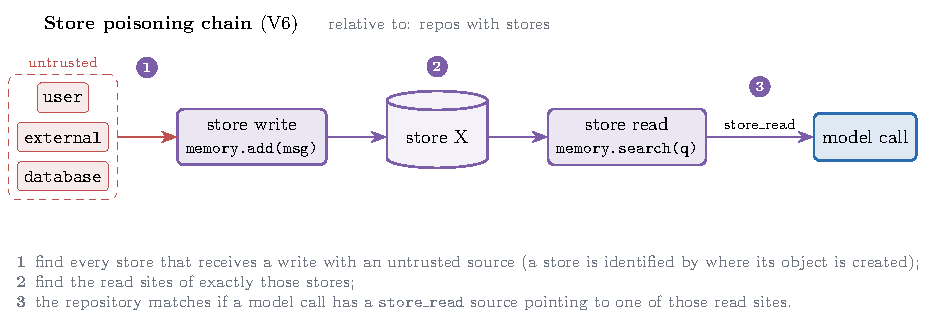
\includegraphics[width=\linewidth]{Images/flow/risk_store_chain.pdf}
  \caption{Detection of the store poisoning chain in three steps.}
  \label{fig:risk-store}
\end{figure}

\begin{table}[t]
\centering
\footnotesize
\renewcommand{\arraystretch}{1.25}
\setlength{\tabcolsep}{4pt}
\caption{Risk patterns, the attack vectors (V) and risks (R) they are preconditions for, and the repositories they are reported relative to.}
\label{tab:df-patterns}
\begin{tabular}{@{}>{\raggedright\arraybackslash}p{0.47\textwidth}>{\raggedright\arraybackslash}p{0.12\textwidth}>{\raggedright\arraybackslash}p{0.08\textwidth}>{\raggedright\arraybackslash}p{0.23\textwidth}@{}}
\toprule
\textbf{Pattern: a repository matches when\ldots} & \textbf{Vectors} & \textbf{Risks} & \textbf{Relative to} \\
\midrule
\emph{Untrusted to model}: user, external, or database content reaches a model call & V4, V1 & R2 & repositories with model calls \\
\emph{Indirect to model}: external, retrieved, or tool content reaches a model call & V1 & R2, R3 & repositories with model calls \\
\emph{Untrusted to instructions}: untrusted or indirect content reaches instructions or a system message & V1, V4 & R2 & repositories with model inputs \\
\emph{Tool risk combination}: a tool returns external, database, or retrieved content, and a tool has a command or file-system effect & V1, V3 & R6 & repositories with tools \\
\emph{Store poisoning chain}: untrusted content is written to a store whose retrieved content reaches a model call & V6 & R3, R6 & repositories with stores \\
\bottomrule
\end{tabular}
\end{table}

% =============================================================================
\section{Validation}
\label{sec:df-validation}

\emph{Recall} is measured on manually inspected repositories: every model call is identified by hand, and we count how many the analysis finds. \emph{Precision} is measured on a random sample of findings, stratified by repository: for each sampled input we check whether the sink is real and whether its sources are correct, separately for confirmed and heuristic detections. In addition, every analysis rule has a small example repository with a fixed expected output; every change to the analysis was checked against all of them, so that an improvement for one pattern cannot silently change the results for another. Results are reported in Section~\ref{sec:res-rq4}.

% =============================================================================
\section{Limitations}
\label{sec:df-limitations}

The analysis under-approximates data flows in several known situations, so most of its counts are lower bounds. The most consequential limitation concerns what tools do with the input the model gives them.

\paragraph{Effects outside the tool body.} Tool effects, command execution, file access, network requests, and database operations, are only searched for directly in the body of a tool function. Tools, however, often delegate their work to helper functions in the application, and the model-chosen arguments are passed on to them. In one of the repositories inspected during validation, an image-generation tool passes its \texttt{prompt} parameter, chosen by the model, to a helper function, which forwards it to a provider object that sends it to an external image-generation service. The network request that carries the model's input is made inside the helper, not in the tool's body, and is therefore not recorded as an effect. The tool's parameters are still recorded (as \texttt{model} sources), and its return value is still traced through the helper; what is missed is that the model's input leaves the application. The numbers of tools with command, file, network, and database effects, and with them the tool risk combination, are therefore lower bounds, and they can only be too low, never too high. Extending the search for effects to the helper functions a tool calls---as the backward tracing already does for return values---would require a new run over the corpus and a new validation, and was not possible within the time available for this thesis; it is discussed as future work (Chapter~\ref{chap:conclusion}).

\paragraph{Objects selected at run time.} The same example shows a second, related limitation. The provider object that calls the external service is chosen at run time from a registry of providers (here selected by the name \texttt{"volces"}). Because the analysis cannot determine statically which class the object belongs to, it cannot follow the call into the provider's code: the trace stops at that point, and the part of the tool's result that comes from the external service---which in reality depends on the model's prompt---is reported as undetermined rather than as \texttt{external} content. Plugin registries, provider maps, and other forms of dynamic dispatch are common in agentic applications, and they contribute to the undetermined shares reported in Chapter~\ref{chap:results}.

\paragraph{Other under-approximations.} Functions only called from outside the repository (such as public library functions) have no call sites to trace; state managed by frameworks or user interfaces (a LangGraph state, a Streamlit session) and data passed through callbacks, queues, or events are not followed; database writes are not tracked; dispatch through \texttt{if}/\texttt{switch} on a tool name is not detected; and stores filled outside the repository cannot be linked to their writes. Two repositories of the selected subset could not be analysed because they no longer exist on GitHub.

\paragraph{Test files.} Folders of tests are skipped during the scan, but many projects keep test files next to the source code (\texttt{*.test.ts}, \texttt{test\_*.py}). The validation found sinks inside such files and application functions whose sources were partly taken from test call sites. Test files are therefore removed from the results after the scan: their sinks and source occurrences are dropped, trace ends inside them are removed, and the affected values are classified again with the same rules. Including them changes each risk pattern by at most one repository, but inflates the share of static inputs, because test fixtures pass fixed prompts and documents to the applications' AI components.

\paragraph{Over-approximations and broad definitions.} The analysis may over-approximate where heuristic sinks are not AI sinks (hence reported separately) and where identifiers such as session identifiers passed to a store are counted as written content. Finally, two source definitions are deliberately broad: files read from a non-fixed path count as \texttt{external}, and command-line arguments as \texttt{user} input.